\achapter{29}{The Singular Value Decomposition} \label{chap:SVD}

\vspace*{-17 pt}
\framebox{
\parbox{\dimexpr\linewidth-3\fboxsep-3\fboxrule}
{\begin{fqs}
\item What is the operator norm of a matrix and what does it tell us about the matrix? 
\item What is a singular value decomposition of a matrix? Why is a singular value decomposition important?  
\item How does a singular value decomposition relate fundamental subspaces connected to a matrix?  
\item What is an outer product decomposition of a matrix and how is it useful? 
\end{fqs}}}% \hspace*{3 pt}}

\vspace*{13 pt}

\csection{Application: Search Engines and Semantics}    
\label{sec:appl_search_engn} 

Effective search engines search for more than just words. Language is complex and search engines must deal with the fact that there are often many ways to express a given concept (this is called \emph{synonymy}, that multiple words can have the same meaning), and that a single word can have multiple meanings (\emph{polysemy}). As a consequence, a search on a word may provide irrelevant matches (e.g., searching for \emph{derivative} could provide pages on mathematics or financial securities) or you might search for articles on \emph{cats} but the paper you really want uses the word \emph{felines}.  A better search engine will not necessarily try to match terms, but instead retrieve information based on concept or intent. Latent Semantic Indexing (LSI)\index{Latent Semantic Indexing} (or \emph{Latent Semantic Analysis}), developed in the late 1980s, helps search engines determine concept and intent in order to provide more accurate and relevant results. LSI essentially works by providing underlying (latent) relationships between words (semantics) that search engines need to provide context and understanding (indexing). LSI provides a mapping of both words and documents into a lower dimensional  ``concept" space, and makes the search in this new space. The mapping is provided by the  singular value decomposition. 

\csection{Introduction}
\label{sec:svd_intro}

The singular value decomposition (SVD) of a matrix is an important and useful matrix decomposition. Unlike other matrix decompositions, \emph{every} matrix has a singular value decomposition. The SVD is used in a variety of applications including scientific computing, digital signal processing, image compression, principal component analysis, web searching through latent semantic indexing, and seismology. 
%http://www.math.pitt.edu/~sussmanm/2071/lab09/
Recall that the eigenvector decomposition of an $n \times n$ diagonalizable matrix $M$ has the form $P^{-1}MP$, where the columns of the matrix $P$ are $n$ linearly independent eigenvectors of $M$ and the diagonal entries of the diagonal matrix $P^{-1}MP$ are the eigenvalues of $M$. The singular value decomposition does something similar for any matrix of any size. One of the keys to the SVD is that the matrix $A^{\tr}A$ is symmetric for any matrix $A$. 


\csection{The Operator Norm of a Matrix}
\label{sec:mtx_op_norm}

Before we introduce the Singular Value Decomposition, let us work through some preliminaries to motivate the idea. The first is to provide an answer to the question ``How `big' is a matrix?" There are many ways to interpret and answer this question, but a substantial (and useful) answer should involve more than just the dimensions of the matrix. A good measure of the size of a matrix, which we will refer to as the norm of the matrix, should take into account the action of the linear transformation defined by the matrix on vectors. This then will lead to questions about how difficult or easy is it to solve a matrix equation $A \vx = \vb$.

If we want to incorporate the action of a matrix $A$ into a calculation of the norm of $A$, we might think of measuring how much $A$ can change a vector $\vx$. This could lead us to using $||A\vx||$ as some sort of measure of a norm of $A$. However, since $||A (c\vx)|| = |c| \ ||A\vx||$ for any scalar $c$, scaling $\vx$ by a large scalar will produce a large norm, so this is not a viable definition of a norm. We could instead measure the \emph{relative} effect that $A$ has on a vector $\vx$ as $\ds \frac{||A\vx||}{||\vx||}$, since this ratio does not change when $\vx$ is multiplied by a scalar. The largest of all of these ratios would provide a good sense of how much $A$ can change vectors. Thus, we define the operator norm of a matrix $A$ as follows.

\begin{definition} The \textbf{operator norm}\index{operator norm of a matrix}\footnote{Technically this definition should be in terms of a supremum, but because the equivalent definition restricts the $\vx$'s to a compact subset, the sup is achieved and we can use max.} of a matrix $A$ is  
\[||A|| = \max_{||\vx|| \neq 0} \left\{\frac{||A\vx||}{||\vx||} \right\}.\]
\end{definition}

Due to the linearity of matrix multiplication, we can restrict ourselves to unit vectors for an equivalent definition of the operator norm of the matrix $A$ as
\[||A|| = \ds \max_{||\vx|| = 1}\{||A\vx||\}.\]

\begin{pa} \label{pa:7_c_1} ~
\be
	\item Determine $||A||$ if $A$ is the zero matrix. 

\item Determine $||I_n||$, where $I_n$ is the $n \times n$ identity matrix. 


\item Let $A = \left[ \begin{array}{cc} 1&0\\0&2 \end{array} \right]$. Find $||A||$. Justify your answer. (Hint: $x_1^2+4x_2^2 \leq 4(x_1^2 + x_2^2)$.)


\item  If $P$ is an orthogonal matrix, what is $||P||$? Why?

 
\ee
\end{pa}


The operator norm of a matrix tells us that how big the action of an $m \times n$ matrix is can be determined by its action on the unit sphere in $\R^n$ (the unit sphere is the set of terminal point of unit vectors). Let us consider two examples.

\begin{example} Let $A = \left[ \begin{array}{cc} 2&1 \\ 2&5 \end{array} \right]$. We can draw a graph to see the action of $A$ on the unit circle. A picture of the set $\{A\vx \ : \ ||\vx|| = 1\}$ is shown in Figure \ref{F:7_c_Mat_norm1}.
\begin{figure}[h]
\begin{center}
\resizebox{!}{2.0in}{\includegraphics{7_c_Mat_norm_a}}
%\resizebox{!}{2.0in}{\includegraphics{7_c_Mat_norm1}} \hspace{0.5in} \resizebox{!}{2.0in}{\includegraphics{7_c_Op_norm_1}}
\end{center}
\caption{The image of the unit circle under the action of $A$.}
\label{F:7_c_Mat_norm1}
\end{figure}

It appears that $A$ transforms the unit circle into an ellipse. To find $||A||$ we want to maximize $||A\vx||$ for $\vx$ on the unit circle. This is the same as maximizing
\[||A\vx||^2 = (A\vx)^{\tr}(A\vx) = \vx^{\tr}A^{\tr}A\vx.\]
Now $A^{\tr}A = \left[ \begin{array}{cc} 8&12 \\ 12&26 \end{array} \right]$ is a symmetric matrix, so we can orthogonally diagonalize $A^{\tr}A$. The eigenvalues of $A^{\tr}A$ are 32 and 2. Let $P = [\vu_1 \ \vu_2]$, where $\vu_1=\left[ \frac{\sqrt{5}}{5} \ \frac{2\sqrt{5}}{5} \right]^{\tr}$ is a unit eigenvector of $A^{\tr}A$ with eigenvalue 32 and $\vu_2=\left[ -\frac{2\sqrt{5}}{5} \ \frac{\sqrt{5}}{5} \right]^{\tr}$ is a unit eigenvector of $A^{\tr}A$ with eigenvalue 2. Then $P$ is an orthogonal matrix such that $P^{\tr}(A^{\tr}A)P = \left[ \begin{array}{cc} 32&0 \\ 0&2 \end{array} \right] = D$. It follows that 
\[\vx^{\tr} (A^{\tr}A)  \vx = \vx^{\tr} PDP^{\tr} \vx = (P^{\tr}\vx)^{\tr} D (P^{\tr}\vx).\]
Now $P^{\tr}$ is orthogonal, so $||P^{\tr}\vx|| = ||\vx||$ and $P^{\tr}$ maps the unit circle to the unit circle. Moreover, if $\vx$ is on the unit circle, then $\vy = P\vx$ is also on the unit circle and $P^{\tr}\vy = P^{\tr}P\vx = \vx$. So every point $\vx$ on the unit circle corresponds to a point $P\vx$ on the unit circle. Thus, the forms $\vx^{\tr} (A^{\tr}A)  \vx$ and $(P^{\tr}\vx)^{\tr} D (P^{\tr}\vx)$ take on exactly the same values over all points on the unit circle. Now we just need to find the maximum value of $(P^{\tr}\vx)^{\tr} D (P^{\tr}\vx)$. This turns out to be relatively easy since $D$ is a diagonal matrix.

Let's simplify the notation. Let $\vy = P^{\tr}\vx$. Then our job is to maximize $\vy^{\tr}D\vy$. If $\vy = [y_1 \ y_2]^{\tr}$, then
\[\vy^{\tr} D  \vy = 32y_1^2 + 2y_2^2.\]
We want to find the maximum value of this expression for $\vy$ on the unit circle. Note that $2y_2^2 \leq 32y_2^2$ and so 
\[32y_1^2 + 2y_2^2 \leq 32y_1^2 + 32y_2^2 = 32(y_1^2+y_2^2) = 32||\vy||^2 = 32.\]
Since $[1 \ 0]^{\tr}$ is on the unit circle, the expression $32y_1^2 + 2y_2^2$ attains the value 32 at some point on the unit circle, so 32 is the maximum value of $\vy^{\tr} D \vy$ over all $\vy$ on the unit circle. While we are at it, we can similarly find the minimum value of $\vy^{\tr} D  \vy$ for $\vy$ on the unit circle. Since $2y_1^2 \leq 32y_1^2$ we see that 
\[32y_1^2 + 2y_2^2 \geq 2y_1^2 + 2y_2^2 = 2(y_1^2+y_2^2) = 2||\vy||^2 = 2.\]
Since the expression $\vy^{\tr} D \vy$ attains the value 2 at $[0 \ 1]^{\tr}$  on the unit circle, we can see that $\vy^{\tr} D \vy$ attains the minimum value of 2 on the unit circle.

Now we can return to the expression $\vx^{\tr} (A^{\tr}A) \vx$. Since $\vy^{\tr} D \vy$ assumes the same values as $\vx^{\tr} (A^{\tr}A) \vx$, we can say that the maximum value of $\vx^{\tr} (A^{\tr}A) \vx$ for $\vx$ on the unit circle is 32 (and the minimum value is 2). Moreover, the quadratic form $(P^{\tr}\vx)^{\tr} D (P^{\tr}\vx)$ assumes its maximum value when $P^{\tr}\vx = [1 \ 0]^{\tr}$ or $[-1 \ 0]^{\tr}$. Thus, the form $\vx^{\tr} (A^{\tr}A) \vx$ assumes its maximum value at the vector $\vx = P[1 \ 0 ]^{\tr} = \vu_1$ or $-\vu_1$. Similarly, the quadratic form $\vx^{\tr} (A^{\tr}A)  \vx$ attains its minimum value at $P[0 \ 1]^{\tr} = \vu_2$ or $-\vu_2$. We conclude that $||A|| = \sqrt{32}$.

Figure \ref{F:7_c_Mat_norm1_b} shows the image of the unit circle under the action of $A$ and the images of $A\vu_1$ and $A\vu_2$ where $\vu_1, \vu_2$ are the two unit eigenvectors of $A^{\tr}A$. The image also supports that $A\vx$ assumes its maximum and minimum values for points on the unit circle at $\vu_1$ and $\vu_2$.
\begin{figure}[h]
\begin{center}
\resizebox{!}{2.0in}{
\includegraphics{7_c_Mat_norm_b}}
%\resizebox{!}{2.0in}{\includegraphics{7_c_Mat_norm1}} \hspace{0.5in} \resizebox{!}{2.0in}{\includegraphics{7_c_Op_norm_1}}
\end{center}
\caption{The image of the unit circle under the action of $A$, and the vectors $A\vu_1$ and $A\vu_2$}
\label{F:7_c_Mat_norm1_b}
\end{figure}
\end{example}


\noindent \textbf{IMPORTANT NOTE 1:} What we have just argued is that the maximum value of $||A\vx||$ for $\vx$ on the unit sphere in $\R^n$ is the square root of the largest eigenvalue of $A^{\tr}A$ and occurs at a corresponding unit eigenvector.

\begin{example} This same process works for matrices other than $2 \times 2$ ones. For example, consider $A = \left[ \begin{array}{rrr} -2&8&20 \\ 14&19&10 \end{array} \right]$. In this case $A$ maps $\R^3$ to $\R^2$. The image of the unit sphere $\{\vx \in \R^3  : ||\vx|| = 1\}$ under left multiplication by $A$ is a filled ellipse as shown in Figure \ref{F:7_c_Mat_norm_2}.
\begin{figure}[h]
\begin{center}
\resizebox{!}{2.0in}{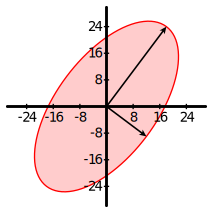
\includegraphics{7_c_Mat_norm_2}}
%\resizebox{!}{2.0in}{\includegraphics{7_c_Mat_norm1}} \hspace{0.5in} \resizebox{!}{2.0in}{\includegraphics{7_c_Op_norm_1}}
\end{center}
\caption{The image of the unit circle under the action of $A$, and the vectors $A\vu_1$ and $A\vu_2$}
\label{F:7_c_Mat_norm_2}
\end{figure}
As with the previous example, the norm of $A$ is the square root of the maximum value of $\vx^{\tr} (A^{\tr}A) \vx$ and this maximum value is the dominant eigenvalue of $A^{\tr}A =  \left[ \begin {array}{ccc} 200&250&100\\ \noalign{\medskip}250&425&350\\ \noalign{\medskip}100&350&500\end {array} \right]$. The eigenvalues of $A$ are $\lambda_1 = 900$, $\lambda_2 = 225$, and $\lambda_3 = 0$ with corresponding unit eigenvectors $\vu_1=\left[ \frac{1}{3} \ \frac{2}{3} \ \frac{2}{3} \right]^{\tr}$, $\vu_1=\left[ -\frac{2}{3} \ -\frac{1}{3} \ \frac{2}{3} \right]^{\tr}$, and $\vu_3=\left[ \frac{2}{3} \ -\frac{2}{3} \ \frac{1}{3} \right]^{\tr}$. So in this case we have $||A|| = \sqrt{900} = 30$. The transformation defined by matrix multiplication by $A$ from $\R^3$ to $\R^2$ has a one-dimensional kernel which is spanned by the eigenvector corresponding to $\lambda_3$. The image of the transformation is 2-dimensional and the image of the unit circle is an ellipse where $A\vu_1$ gives the major axis of the ellipse and $A\vu_2$ gives the minor axis. Essentially, the square roots of the eigenvalues of $A^{\tr}A$ tell us how $A$ stretches the image space in each direction.
\end{example}


\noindent \textbf{IMPORTANT NOTE 2:} We have just argued that the image of the unit $n$-sphere under the action of an $m \times n$ matrix is an ellipsoid in $\R^m$ stretched the greatest amount, $\sqrt{\lambda_1}$, in the direction of an eigenvector for the largest eigenvalue ($\lambda_1$) of $A^{\tr}A$; the next greatest amount, $\sqrt{\lambda_2}$, in the direction of a unit vector for the second largest eigenvalue ($\lambda_2$) of $A^{\tr}A$; and so on.


\begin{activity}  Let $A = \left[ \begin{array}{rc} 0&5\\ 4&3 \\ -2&1\end{array} \right].$ Then $A^{\tr}A = \left[ \begin{array}{cc} 20&10\\ 10&35\end{array}
 \right]$. The eigenvalues of $A^{\tr}A$ are $\lambda_1 = 40$ and $\lambda_2 = 15$ with respective eigenvectors $\vv_1 = \left[ \begin{array}{c} \frac{1}{2} \\ 1 \end{array} \right]$ and $\vv_2 = \left[ \begin{array}{r} -2 \\ 1 \end{array} \right]$.
 	\ba
	\item Find $||A||$.
	
	\item Find a unit vector $\vx$ at which $||A\vx||$ assumes its maximum value.
	
	\ea
\end{activity}


%\begin{activity} Let $A$ be a symmetric matrix.
%	\ba
%	\item Let $\lambda$ be an eigenvalue of $A$ with eigenvector $\vv$. Show that $\lambda^2$ is an eigenvalue of $A^2$.
	
	
%	\item How are the eigenvalues of $A$ related to the eigenvalues of $A^{\tr}A$?	

	
%	\ea
%\end{activity}


\csection{The SVD}
\label{sec:svd}

The Singular Value Decomposition (SVD) is essentially a concise statement of what we saw in the previous section that works for \emph{any} matrix. We will uncover the SVD in this section.

\begin{pa} \label{pa:7_c_2} Let $A = \left[ \begin{array}{ccc} 1&1&0\\ 0&1&1 \end{array} \right]$. Since $A$ is not square, we cannot diagonalize $A$. However, the matrix
\[A^{\tr}A = \left[ \begin{array}{ccc} 1&1&0 \\ 1&2&1 \\ 0&1&1 \end{array} \right]\]
is a symmetric matrix and can be orthogonally diagonalized. The eigenvalues of $A^{\tr}A$ are 3, 1, and 0 with corresponding eigenvectors
\[\left[ \begin{array}{c} 1\\2\\1 \end{array} \right], \ \left[ \begin{array}{r} -1\\0\\1 \end{array} \right], \ \text{ and } \ \left[ \begin{array}{r} 1\\-1\\1 \end{array} \right],\]
respectively. Use appropriate technology to do the following. 
\be
\item Find an orthogonal matrix $V = [\vv_1 \ \vv_2 \ \vv_3]$ that orthogonally diagonalizes $A^{\tr}A$, where
\[V^{\tr}\left(A^{\tr}A\right)V = \left[ \begin{array}{ccc} 3&0&0\\0&1&0\\0&0&0 \end{array} \right].\]


\item For $i=1,2$, let $\vu_i = \frac{A \vv_i}{||A \vv_i||}$. Find each $\vu_i$. Why don't we define $\vu_3$ in this way?


\item Let $U = [\vu_1 \ \vu_2]$. What kind of matrix is $U$? Explain.


\item  Calculate the matrix product $U^{\tr}AV$. What do you notice? How is this similar to the eigenvector decomposition of a matrix?

 
\ee
\end{pa}


Preview Activity \ref{pa:7_c_2} contains the basic ideas behind the Singular Value Decomposition. Let $A$ be an $m \times n$ matrix with real entries. Note that $A^{\tr}A$ is a symmetric $n \times n$ matrix and, hence, it can be orthogonally diagonalized. Let $V = [\vv_1 \ \vv_2 \ \vv_3 \  \cdots \  \vv_n ]$ be an $n \times n$ orthogonal matrix whose columns form an orthonormal set of eigenvectors for $A^{\tr}A$. For each $i$, let $(A^{\tr}A)\vv_i = \lambda_i \vv_i$. We know
\[V^{\tr} (A^{\tr}A) V = \left[ \begin{array}{ccccc} \lambda_1&0&0&\cdots&0 \\ 0& \lambda_2&0&\cdots&0 \\ \vdots & \vdots & \vdots & & \vdots  \\ 0&0&0&\cdots& \lambda_n \end{array} \right].\]

Now notice that for each $i$ we have
\begin{equation}
|| A \vv_i ||^2 = (A\vv_i)^{\tr}(A\vv_i) = \vv_i^{\tr}(A^{\tr}A) \vv_i = \vv_i^{\tr} \lambda_i \vv_i = \lambda_i ||\vv_i||^2 = \lambda_i, \label{eq:7_c_sing_vals1}
\end{equation}
so $\lambda_i \geq 0$. Thus, the matrix $A^{\tr}A$ has no negative eigenvalues. We can always arrange the eigenvectors and eigenvalues of $A^{\tr}A$ so that
\[\lambda_1 \geq \lambda_2 \geq \cdots \geq \lambda_n \geq 0.\]

Also note that
\[(A\vv_i) \cdot (A\vv_j) = (A\vv_i)^{\tr} (A\vv_j) = \vv_i^{\tr} (A^{\tr}A) \vv_j = \vv_i^{\tr} \lambda_j\ \vv_j = \lambda_j \vv_i \cdot \vv_j = 0\]
if $i \neq j$. So the set $\{A\vv_1, A\vv_2, \ldots, A\vv_n\}$ is an orthogonal set in $\R^m$. Each of the vectors $A\vv_i$ is in $\Col A$, and so $\{A\vv_1, A\vv_2, \ldots, A\vv_n\}$ is an orthogonal subset of $\Col A$. It is possible that $A\vv_i = \vzero$ for some of the $\vv_i$ (if $A^{\tr}A$ has 0 as an eigenvalue). Let $\vv_1$, $\vv_2$, $\ldots$, $\vv_r$ be the eigenvectors corresponding to the nonzero eigenvalues. Then the set
\[\CB=\{A\vv_1, A\vv_2, \ldots, A\vv_r\}\]
is a linearly independent set of nonzero orthogonal vectors in $\Col A$. Now we will show that $\CB$ is a basis for $\Col A$. Let $\vy$ be a vector in $\Col A$. Then $\vy = A\vx$ for some vector $\vx$ in $\R^n$. Recall that the vectors $\vv_1$, $\vv_2$, $\ldots$, $\vv_n$ form an orthonormal basis of $\R^n$, so
\[\vx = x_1 \vv_1 + x_2 \vv_2 + \cdots + x_n \vv_n\]
for some scalars $x_1$, $x_2$, $\ldots$, $x_n$. Since $A\vv_j = \vzero$ for $r+1 \leq j \leq n$ we have
\begin{align*}
\vy &= A\vx \\
	&= A(x_1 \vv_1 + x_2 \vv_2 + \cdots + x_n \vv_n) \\
	&= x_1 A\vv_1 + x_2 A\vv_2 + \cdots + x_r A\vv_r + x_{r+1} A \vv_{r+1} + \cdots + x_n A\vv_n \\
	&= x_1 A\vv_1 + x_2 A\vv_2 + \cdots + x_r A\vv_r.
\end{align*}
So $\Span \ \CB = \Col A$ and $\CB$ is an orthogonal basis for $\Col A$.

Now we are ready to find the Singular Value Decomposition of $A$. First we create an orthonormal basis $\{\vu_1, \vu_2, \ldots, \vu_r\}$ for $\Col A$ by normalizing the vectors $A\vv_i$. So we let
\[\vu_i = \frac{A\vv_i}{||A\vv_i||}\]
for $i$ from 1 to $r$.

Remember from (\ref{eq:7_c_sing_vals1}) that $||A\vv_i||^2 = \lambda_i$, so if we let $\sigma_i = \sqrt{\lambda_i}$, then we have
\[\vu_i = \frac{A\vv_i}{\sigma_i} \text{ and } A \vv_i = \sigma_i \vu_i.\]
We ordered the $\lambda_i$ so that $\lambda_1 \geq \lambda_2 \geq \cdots \geq \lambda_n$, so we also have
\[\sigma_1 \geq \sigma_2 \geq \cdots \geq \sigma_r > 0.\]
The scalars $\sigma_1$, $\sigma_2$, $\ldots$, $\sigma_n$ are called the \emph{singular values} of $A$.

\begin{definition} Let $A$ be an $m \times n$ matrix. The \textbf{singular values}\index{singular values} of $A$ are the square roots of the eigenvalues of $A^{\tr}A$. 
\end{definition} 

The vectors $\vu_1$, $\vu_2$, $\ldots$, $\vu_r$ are $r$ orthonormal vectors in $\R^m$. We can extend the set $\{\vu_1$, $\vu_2$, $\ldots$, $\vu_r\}$ to an orthonormal basis $\CC = \{\vu_1, \vu_2, \ldots, \vu_r, \vu_{r+1} \vu_{r+2}, \ldots, \vu_m\}$ of $\R^m$. Recall that $A \vv_i = \sigma_i \vu_i$ for $1 \leq i \leq r$ and $A \vv_j = \vzero$ for $r+1 \leq j \leq n$, so
\begin{align*}
AV &= A [\vv_1 \  \vv_2  \ \cdots  \ \vv_n] \\
	&= [A\vv_1  \ A\vv_2  \ \cdots  \ A\vv_n] \\
	&= [\sigma_1 \vu_1  \ \sigma_2 \vu_2  \ \cdots  \ \sigma_r \vu_r  \ \vzero  \ \vzero  \ \cdots  \ \vzero].
\end{align*}
We can write the matrix $[\sigma_1 \vv_1  \ \sigma_2 \vv_2  \ \cdots  \ \sigma_r \vv_r  \ \vzero  \ \vzero  \ \cdots  \ \vzero]$ in another way. Let $\Sigma$ be the $m\times n$ matrix defined as
\[\Sigma = \left[ \begin{array}{ccccc|c} \sigma_1&&&&0& \\ & \sigma_2&&&&0 \\ && \sigma_3&&& \\ &  & & \ddots & & \\ 0&&&& \sigma_r \\ \hline &&0&&&0 \end{array} \right].\]
Now
\[[\vu_1  \ \vu_2  \ \cdots  \ \vu_m] \Sigma = [\sigma_1\vu_1  \ \sigma_1\vu_2  \ \cdots  \ \sigma_r\vu_r \ \vzero \ \vzero \ \cdots \ \vzero] = AV.\]
So if $U = [\vu_1 \ \vu_2 \ \cdots \ \vu_m]$, then
\[U\Sigma = AV.\]
Since $V$ is an orthogonal matrix, we have that
\[U \Sigma V^{\tr} = AV V^{\tr} = A.\]
This is the Singular Value Decomposition of $A$.



\begin{theorem}[The Singular Value Decomposition] Let $A$ be an $m \times n$ matrix of rank $r$. There exist an $m \times m$ orthogonal matrix $U$, an $n \times n$ orthogonal matrix $V$, and an $m \times n$ matrix $\Sigma$ whose first $r$ diagonal entries are the singular values $\sigma_1$, $\sigma_2$, $\ldots$, $\sigma_r$ and whose other entries are 0, such that
\[A = U \Sigma V^{\tr}.\]
\end{theorem}



 \noindent \textbf{SVD Summary: } A Singular Value Decomposition of an $m \times n$ matrix $A$ of rank $r$ can be found as follows.
	\begin{enumerate}
	\item Find an orthonormal basis $\{\vv_1, \vv_2, \vv_3, \ldots, \vv_n\}$ of eigenvectors of $A^{\tr}A$ such that $(A^{\tr}A) \vv_i = \lambda_i \vv_i$ for $i$ from 1 to $n$ with $\lambda_1 \geq \lambda_{2} \geq \cdots \geq \lambda_n \geq 0$ with the first $r$ eigenvalues being positive. The vectors $\vv_1$, $\vv_2$, $\vv_3$, $\ldots$, $\vv_n$ are the \emph{right singular vectors}\index{singular vectors!right} of $A$.
	\item Let
\[V= [\vv_1 \  \vv_2 \  \vv_3 \  \cdots \  \vv_n ].\]
Then $V$ orthogonally diagonalizes $A^{\tr}A$.
	\item The singular values of $A$ are the numbers $\sigma_i$, where $\sigma_i = \sqrt{\lambda_i} > 0$ for $i$ from 1 to $r$. Let $\Sigma$ be the $m \times n$ matrix 
\[\Sigma = \left[ \begin{array}{ccccc|c} \sigma_1&&&&0& \\ & \sigma_2&&&&0 \\ && \sigma_3&&& \\ &  & & \ddots & & \\ 0&&&& \sigma_r \\ \hline &&0&&&0 \end{array} \right] \]
	\item For $i$ from 1 to $r$, let $\vu_i = \frac{A\vv_i}{||A\vv_i||}$. Then the set $\{\vu_1, \vu_2, \ldots, \vu_r\}$ forms an orthonormal basis of $\Col A$.
	\item Extend the set $\{\vu_1, \vu_2, \ldots, \vu_r\}$ to an orthonormal basis 
\[\{\vu_1, \vu_2, \ldots, \vu_r, \vu_{r+1} \vu_{r+2}, \ldots, \vu_m\}\]
of $\R^m$. Let
\[U = [\vu_1 \ \vu_2 \ \cdots \ \vu_m].\]
The vectors $\vu_1$, $\vu_2$, $\ldots$, $\vu_m$ are the \emph{left singular vectors}\index{singular vectors!left} of $A$.
	\item Then $A = U \Sigma V^{\tr}$ is a singular value decomposition of $A$.
	\end{enumerate}



\begin{activity} \label{ex:7_c_SVD} Let $A = \left[ \begin {array}{rc} 0&5\\ \noalign{\medskip}4&3
\\ \noalign{\medskip}-2&1\end {array} \right].$ Then $A^{\tr}A = \left[ \begin {array}{cc} 20&10\\ \noalign{\medskip}10&35\end {array}
 \right]$. The eigenvalues of $A^{\tr}A$ are $\lambda_1 = 40$ and $\lambda_2 = 15$ with respective eigenvectors $\vw_1 = \left[ \begin {array}{c} 1 \\ 2 \end {array} \right]$ and $\vw_2 = \left[ \begin {array}{r} -2 \\ 1 \end {array} \right]$.
 	\ba
	\item Find an orthonormal basis $\{\vv_1, \vv_2, \vv_3, \ldots, \vv_n\}$ of eigenvectors of $A^{\tr}A$. What is $n$? Find the matrix $V$ in a SVD for $A$.
		
	
	
	\item Find the singular values of $A$. What is the rank $r$ of $A$? Why?

	
	
	\item What are the dimensions of the matrix $\Sigma$ in a SVD of $A$? Find $\Sigma$.
	
	
	
	\item Find the vectors $\vu_1$, $\vu_2$, $\ldots$, $\vu_r$. If necessary, extend this set to an orthonormal basis
\[\{\vu_1, \vu_2, \ldots, \vu_r, \vu_{r+1} \vu_{r+2}, \ldots, \vu_m\}\]
of $\R^m$. 
	
	
	
	\item Find the matrix $U$ so that $A = U \Sigma V^{\tr}$ is a SVD for $A$.
	
	
	
	\ea
\end{activity}

There is another way we can write this SVD of $A$. Let the $m \times n$ matrix $A$ have a singular value decomposition $U \Sigma V^{\tr}$, where
\begin{align*}
U &= [\vu_1 \ \vu_2 \ \cdots \ \vu_m], \\
\Sigma &= \left[ \begin{array}{ccccc|c} \sigma_1&&&&0& \\ & \sigma_2&&&&0 \\ && \sigma_3&&& \\ &  & & \ddots & & \\ 0&&&& \sigma_r \\ \hline &&0&&&0 \end{array} \right],  \text{ and }  \\
V &= [\vv_1 \ \vv_2 \ \vv_3 \   \cdots \  \vv_n ].
\end{align*}

Since $A = U \Sigma V^{\tr}$ we see that
\begin{align}
A &= [ \vu_1 \ \vu_2 \ \vu_3 \ \cdots \ \vu_m] \left[ \begin{array}{ccccc|c} \sigma_1&&&&0& \\ & \sigma_2&&&&0 \\ && \sigma_3&&& \\ &  & & \ddots & & \\ 0&&&& \sigma_r \\ \hline &&0&&&0 \end{array} \right] \left[ \renewcommand{\arraystretch}{1.2} \begin{array}{c} \vv_1^{\tr} \\ \vv_2^{\tr} \\ \vv_3^{\tr} \\ \vdots \\ \vv_n^{\tr} \end{array} \right] \notag \\
	&= [ \sigma_1\vu_1 \ \sigma_2\vu_2 \ \sigma_3\vu_3 \ \cdots \ \sigma_r\vu_r \ \vzero \ \cdots \ \vzero] \left[ \renewcommand{\arraystretch}{1.2} \begin{array}{c} \vv_1^{\tr} \\ \vv_2^{\tr} \\ \vv_3^{\tr} \\ \vdots \\ \vv_n^{\tr} \end{array} \right] \notag \\
	&= \sigma_1 \vu_1\vv_1^{\tr} + \sigma_2 \vu_2\vv_2^{\tr} + \sigma_3 \vu_3\vv_3^{\tr} + \cdots + \sigma_r \vu_r\vv_r^{\tr}. \label{eq:7_c_SVD}
\end{align}
This is called an \emph{outer product decomposition}\index{outer product decomposition} of $A$ and tells us everything we learned above about the action of the matrix $A$ as a linear transformation. Each of the products $\vu_i\vv_i^{\tr}$ is a rank 1 matrix (see Exercise \ref{ex:7_c_rank1}), and $||A\vv_1|| = \sigma_1$ is the largest value $A$ takes on the unit $n$-sphere, $||A\vv_2|| = \sigma_2$ is the next largest dilation of the unit $n$-sphere, and so on. An outer product decomposition allows us to approximate $A$ with smaller rank matrices. For example, the matrix $\sigma_1 \vu_1\vv_1^{\tr}$ is the best rank 1 approximation to $A$, $\sigma_1 \vu_1\vv_1^{\tr} + \sigma_2 \vu_2\vv_2^{\tr} $ is the best rank 2 approximation, and so on. This will be very useful in applications, as we will see in the next section. 

\csection{SVD and the Null, Column, and Row Spaces of a Matrix}
\label{sec:svd_mtx_spaces}

We conclude this section with a short discussion of how a singular value decomposition relates fundamental subspaces of a matrix. We have seen that the vectors $\vu_1$, $\vu_2$, $\ldots$, $\vu_r$ in an SVD for an $m \times n$ matrix $A$ form a basis for $\Col A$. Recall also that $A \vv_j = \vzero$ for $r+1 \leq j \leq n$. Since $\dim(\Nul A) + \dim(\Col A) = n$, it follows that the vectors $\vv_{r+1}$, $\vv_{r+2}$, $\ldots$, $\vv_n$ form a basis for $\Nul A$.  As you will show in the exercises, the set $\{\vv_1, \vv_2, \ldots, \vv_r\}$ is a basis for $\Row A$.  Thus, an SVD for a matrix $A$ tells us about three fundamental vector spaces related to $A$.

%We conclude this section with a short discussion of how a singular value decomposition relates fundamental subspaces of a matrix. Let $A$ be an $m \times n$ matrix with right singular vectors $\vv_1$, $\vv_2$, $\ldots$, $\vv_n$. That is, the set $\{\vv_1, \vv_2, \vv_n\}$ is an orthonormal basis for $\R^n$ consisting of eigenvectors of $A^{\tr}A$. Let $A \vv_i = \lambda_i \v_i$ for $i $from $1$ to $n$, with $\lambda_1 \geq \lambda_2 \geq \cdots \geq \lambda_n \geq 0$, and let $r > 0$ such that $\lambda_i > 0$ for $1 \leq i \leq r$ and $\lambda_j = 0$ for $r+1 \leq j \leq n$. Let $\sigma_i = \sqrt{\lambda_i}$ for $i$ from $1$ to $n$. For $1 \leq i \leq r$, let $\vu_i = \frac{1}{||A \vv_i||}$. The set $\{vu_1, \vu_2, \ldots, \vu_r\}$ is an orthonormal subset of $\R^m$. Extend this set to an orthogonal basis $\{vu_1, \vu_2, \ldots, \vu_r, \vu_{r+1}, \ldots, \vu_m\}$ of $\R^m$. In this context we can relate the four fundamental %subspaces $\Row A$, $\Col A = \Row A^{\tr}$, $\Nul A$, and $\Nul A^{\tr}$.

%\begin{itemize}
%\item We have seen that the set $\{A\vv_1, A\vv_2, \ldots, A\vv_r\}$ is a basis for $\Col A$. Since $A \vv_i = \sigma_i %\vu_i$, it follows that the set $\{\sigma_1 \vu_1, \sigma_2 \vu_2, \ldots, \sigma_r \vu_r\}$ is a basis for $\Col A$. Also, $%\sigma_i > 0$ for each $i$ from $1$ to $r$, so the set $\{\vu_1$, $\vu_2$, $\ldots$, $\vu_r\}$ is an orthonormal basis %for $\Col A$. 

%\item Recall also that $A \vv_j = \vzero$ for $r+1 \leq j \leq n$. Since $\dim(\Nul A) + \dim(\Col A) = n$, it follows that %the set $\{\vv_{r+1}, \vv_{r+2}, \ldots, \vv_n\} is an orthonormal basis for $\Nul A$.  

%\item As you will show in the exercises, the set $\{\vv_1, \vv_2, \ldots, \vv_r\}$ is an orthonormal basis for $\Row A$. 

%\item Finally, since $\dim(\Row A^{\tr}) = \dim(\Col A^{\tr})$, it follows that $\dim(\Nul A^{\tr}) + \dim(\Row A^{\tr}) = m$. %From this we have that the set $\{\vu_{r+1}, \vu_{r+2}, \ldots, \vu_{m\}$ is an orthonormal basis for $\Nul A^{\tr}$. 

%\end{itemize}

%The connections are illustrated in Figure \ref{F:Fundamental_spaces}. Thus, an SVD for a matrix $A$ tells us about %four fundamental vector spaces related to $A$.

%\begin{figure}[h]
%\begin{center}
%\resizebox{!}{2.0in}{\includegraphics{Fundamental_spaces.eps}}
%\end{center}
%\caption{The four fundamental subspaces.}
%\label{F:Fundamental_spaces}
%\end{figure}

\csection{Examples}
\label{sec:svd_exam}

\ExampleIntro

\begin{example} Let $A = \left[ \begin{array}{cccc} 2  &  0  &  0  &  0 \\  0  &  2  &  1  &  0 \\ 0&1  &  2  &  0  \end{array} \right]$. 
\ba
\item Find a singular value decomposition for $A$. You may use technology to find eigenvalues and eigenvectors of matrices. 

\item Use the singular value decomposition to find a basis for $\Col A$, $\Row A$, and $\Nul A$.

\ea


\ExampleSolution
\ba
\item With $A$ as given, we have $A^{\tr}A = \left[ \begin{array}{cccc} 4  &  0  &  0  &  0 \\  0  &  5  &  4  &  0 \\ 0  &  4  &  5  &  0 \\ 0&0&0&0 \end{array} \right]$. Technology shows that the eigenvalues of $A^{\tr}A$ are $\lambda_1 = 9$, $\lambda_2 = 4$, $\lambda_3 = 1$, and $\lambda_4 = 0$ with corresponding orthonormal eigenvectors $\vv_1 = \frac{1}{\sqrt{2}}[0 \ 1 \ 1 \ 0]^{\tr}$, $\vv_2 = [1 \ 0 \ 0 \ 0]^{\tr}$, $\vv_3 = \frac{1}{\sqrt{2}}[0 \ -1 \ 1 \ 0]^{\tr}$, and $\vv_4 = [0 \ 0 \ 0 \ 1]^{\tr}$. This makes $V = [\vv_1 \ \vv_2 \ \vv_3 \ \vv_4]$. The singular values of $A$ are $\sigma_1 = \sqrt{9} = 3$, $\sigma_2 = \sqrt{4}= 2$, $\sigma_3 = \sqrt{1} = 1$, and $\sigma_4 = 0$, so $\Sigma$ is the $3 \times 4$ matrix with the nonzero singular values along the diagonal and zeros everywhere else. Finally, we define the vectors $\vu_i$ as $\vu_i = \frac{1}{||A \vv_i||} A\vv_i$. Again, technology gives us $\vu_1 = \frac{1}{\sqrt{2}}[0 \ 1 \ 1]^{\tr}$, $\vu_2 = [1 \ 0 \ 0]^{\tr}$, and $\vu_3 = \frac{1}{\sqrt{2}}[0 \ -1 \ 1]^{\tr}$. Thus, a singular value decomposition of $A$ is $U \Sigma V^{\tr}$, where 
\begin{align*}
U &= \left[\renewcommand{\arraystretch}{1.2} \begin{array}{ccr} 0&1&0\\ \frac{1}{\sqrt{2}}&0&-\frac{1}{\sqrt{2}} \\ \frac{1}{\sqrt{2}}&0&\frac{1}{\sqrt{2}} \end{array} \right], \\
\Sigma &= \left[ \begin{array}{cccc} 3&0&0&0 \\ 0&2&0&0 \\ 0&0&1&0 \end{array} \right], \ \text{ and } \\
V &= \left[\renewcommand{\arraystretch}{1.2} \begin{array}{ccrc} 0&1&0&0 \\ \frac{1}{\sqrt{2}}&0&-\frac{1}{\sqrt{2}}&0 \\ \frac{1}{\sqrt{2}}&0&\frac{1}{\sqrt{2}}&0 \\ 0&0&0&1 \end{array} \right].
\end{align*}

\item Recall that the right singular vectors of an $m \times n$ matrix $A$ of rank $r$ form an orthonormal basis $\{\vv_1, \vv_2, \vv_3, \ldots, \vv_n\}$ of eigenvectors of $A^{\tr}A$ such that $(A^{\tr}A) \vv_i = \lambda_i \vv_i$ for $i$ from 1 to $n$ with $\lambda_1 \geq \lambda_{2} \geq \cdots \geq \lambda_n \geq 0$. These vectors are the columns of the matrix $V = [\vv_1 \ \vv_2 \ \cdots \ \vv_n]$ in a singular value decomposition of $A$. 

For $i$ from 1 to $r$, we let $\vu_i = \frac{A\vv_i}{||A\vv_i||}$. Then the set $\{\vu_1, \vu_2, \ldots, \vu_r\}$ forms an orthonormal basis of $\Col A$. We extend this set $\{\vu_1, \vu_2, \ldots, \vu_r\}$ to an orthonormal basis $\{\vu_1, \vu_2, \ldots, \vu_r, \vu_{r+1} \vu_{r+2}, \ldots, \vu_m\}$ of $\R^m$.

Recall also that $A \vv_j = \vzero$ for $r+1 \leq j \leq n$. Since $\dim(\Nul A) + \dim(\Col A) = n$, it follows that the vectors $\vv_{r+1}$, $\vv_{r+2}$, $\ldots$, $\vv_n$ form a basis for $\Nul A$.  Finally, the set $\{\vv_1, \vv_2, \ldots, \vv_r\}$ is a basis for $\Row A$. 

So in our example, we have $m = 3$, $n = 4$, $\vv_1 = \frac{1}{\sqrt{2}}[0 \ 1 \ 1 \ 0]^{\tr}$, $\vv_2 = [1 \ 0 \ 0 \ 0]^{\tr}$, $\vv_3 = \frac{1}{\sqrt{2}}[0 \ -1 \ 1 \ 0]^{\tr}$, and $\vv_4 = [0 \ 0 \ 0 \ 1]^{\tr}$. Since the singular values of $A$ are $3$, $2$, $1$, and $0$, it follows that $r = \rank(A) = 3$. We also have $\vu_1 = \frac{1}{\sqrt{2}}[0 \ 1 \ 1]^{\tr}$, $\vu_2 = [1 \ 0 \ 0]^{\tr}$, and $\vu_3 = \frac{1}{\sqrt{2}}[ 0 \ -1 \ 1]^{\tr}$. So 
\[\left\{\frac{1}{\sqrt{2}}[0 \ 1 \ 1 \ 0]^{\tr}, [1 \ 0 \ 0 \ 0]^{\tr}, \frac{1}{\sqrt{2}}[0 \ -1 \ 1 \ 0]^{\tr}\right\}\]
is a basis for $\Row A$ and
\[\{[0 \ 0 \ 0 \ 1]^{\tr}\}\]
is a basis for $\Nul A$. Finally, the set 
\[ \left\{ \frac{1}{\sqrt{2}}[0 \ 1 \ 1]^{\tr}, [1 \ 0 \ 0]^{\tr}, \frac{1}{\sqrt{2}}[[ 0 \ -1 \ 1]^{\tr}\right\}\]
is a basis for $\Col A$. 

\ea


\end{example} 


\begin{example} Let
\[A = \left[ \begin{array}{ccc} 2&5&4\\6&3&0\\6&3&0\\2&5&4 \end{array} \right].\]
The eigenvalues of $A^{\tr}A$ are $\lambda_1 = 144$, $\lambda_2 = 36$, and $\lambda_3=0$ with corresponding eigenvectors
\[\vw_1 = \left[ \begin{array}{c} 2\\2\\1 \end{array} \right], \ \vw_1 = \left[ \begin{array}{r} -2\\1\\2 \end{array} \right], \ \text{ and } \ \vw_1 = \left[ \begin{array}{r} 1\\-2\\2 \end{array} \right].\]
In addition,
\[A \vw_1 = \left[ \begin{array}{c} 18\\18\\18\\18 \end{array} \right] \ \text{ and } A \vw_2 = \left[ \begin{array}{r} 9\\-9\\-9\\9 \end{array} \right].\]
    \ba

    \item Find orthogonal matrices $U$ and $V$, and the matrix $\Sigma$, so that $U \Sigma V^{\tr}$ is a singular value decomposition of $A$.

    \item Determine the best rank 1 approximation to $A$. 
    
    \ea


\ExampleSolution

\ba
\item Normalizing the eigenvectors $\vw_1$, $\vw_2$, and $\vw_3$ to normal eigenvectors $\vv_1$, $\vv_2$, and $\vv_3$, respectively, gives us an orthogonal matrix
\[V = \left[ \renewcommand{\arraystretch}{1.4} \begin {array}{crr} \frac{2}{3}&-\frac{2}{3}&\frac{1}{3}\\ \frac{2}{3}&\frac{1}{3}&-
\frac{2}{3}\\  \frac{1}{3}&\frac{2}{3}&\frac{2}{3}\end {array} \right].\]
Now $A \vv_i = A \frac{\vw_i}{||\vw_i||} = \frac{1}{|| \vw_i ||} A \vw_i$, so normalizing the vectors $A \vv_1$ and $A \vv_2$ gives us vectors \[\vu_1 = \frac{1}{2} \left[ \begin{array}{c} 1\\1\\1\\1\\ \end{array} \right] \ \text{ and } \ \vu_2 = \frac{1}{2} \left[ \begin{array}{r} 1\\-1\\-1\\1\\ \end{array} \right]\]
that are the first two columns of our matrix $U$. Given that $U$ is a $4 \times 4$ matrix, we need to find two other vectors orthogonal to $\vu_1$ and $\vu_2$ that will combine with $\vu_1$ and $\vu_2$ to form an orthogonal basis for $\R^4$. Letting $\vz_1 = [1 \ 1 \ 1 \ 1]^{\tr}$, $\vz_2 = [1 \ -1 \ -1 \ 1]^{\tr}$, $\vz_3 = [1 \ 0 \ 0 \ 0]^{\tr}$, and $\vz_4 = [0 \ 1 \ 0 \ 1]^{\tr}$, a computer algebra system shows that the reduced row echelon form of the matrix $[\vz_1 \ \vz_2 \ \vz_3 \ \vz_4]$ is $I_4$, so that vectors $\vz_1$, $\vz_2$, $\vz_3$, $\vz_4$ are linearly independent. Letting $\vw_1 = \vz_1$ and $\vw_2 = \vz_2$, the Gram-Schmidt process shows that the set $\{\vw_1, \vw_2, \vw_3, \vw_4\}$ is an orthogonal basis for $\R^4$, where 
\begin{align*}
\vw_3 &= [1 \ 0 \ 0 \ 0]^{\tr} - \frac{[1 \ 0 \ 0 \ 0]^{\tr} \cdot [1 \ 1 \ 1 \ 1]^{\tr}}{[1 \ 1 \ 1 \ 1]^{\tr} \cdot [1 \ 1 \ 1 \ 1]^{\tr}} [1 \ 1 \ 1 \ 1]^{\tr} \\
	&\qquad - \frac{[1 \ 0 \ 0 \ 0]^{\tr} \cdot [1 \ -1 \ -1 \ 1]^{\tr}}{[1 \ -1 \ -1 \ 1]^{\tr} \cdot [1 \ -1 \ -1 \ 1]^{\tr}} [1 \ -1 \ -1 \ 1]^{\tr} \\
	&= [1 \ 0 \ 0 \ 0]^{\tr} - \frac{1}{4}[1 \ 1 \ 1 \ 1]^{\tr} - \frac{1}{4} [1 \ -1 \ -1 \ 1]^{\tr} \\
	&= \frac{1}{4} [2 \ 0 \ 0 \ -2]^{\tr}
\end{align*}
and (using $[1 \ 0 \ 0 \ -1]^{\tr}$ for $\vw_3$)
\begin{align*}
\vw_4 &= [0 \ 1 \ 0 \ 0]^{\tr} - \frac{[0 \ 1 \ 0 \ 0]^{\tr} \cdot [1 \ 1 \ 1 \ 1]^{\tr}}{[1 \ 1 \ 1 \ 1]^{\tr} \cdot [1 \ 1 \ 1 \ 1]^{\tr}} [1 \ 1 \ 1 \ 1]^{\tr} \\
	&\qquad - \frac{[0 \ 1 \ 0 \ 0]^{\tr} \cdot [1 \ -1 \ -1 \ 1]^{\tr}}{[1 \ -1 \ -1 \ 1]^{\tr} \cdot [1 \ -1 \ -1 \ 1]^{\tr}} [1 \ -1 \ -1 \ 1]^{\tr} \\
	&\qquad - \frac{[0 \ 1 \ 0 \ 0]^{\tr} \cdot [1 \ 0 \ 0 \ -1]^{\tr}}{[1 \ 0 \ 0 \ -1]^{\tr} \cdot [1 \ 0 \ 0 \ -1]^{\tr}} [1 \ 0 \ 0 \ -1]^{\tr} \\
	&= [0 \ 1 \ 0 \ 0]^{\tr} - \frac{1}{4}[1 \ 1 \ 1 \ 1]^{\tr} + \frac{1}{4} [1 \ -1 \ -1 \ 1]^{\tr} - \vzero \\
	&= \frac{1}{4} [0 \ 2 \ -2 \ 0]^{\tr}.
\end{align*}
The set $\{\vu_1, \vu_2, \vu_3, \vu_4\}$ where $\vu_1 = \frac{1}{2}[1 \ 1 \ 1 \ 1]^{\tr}$, $\vu_2 = \frac{1}{2}[1 \ -1 \ -1 \ 1]^{\tr}$, $\vu_3 = \frac{1}{\sqrt{2}}[1 \ 0 \ 0 \ -1]^{\tr}$ and $\vu_4 = \frac{1}{\sqrt{2}}[0 \ 1 \ -1 \ 0]^{\tr}$ is an orthonormal basis for $\R^4$ and we can let 
\[U = \left[ \renewcommand{\arraystretch}{1.4} \begin{array}{crrr} \frac{1}{2} & \frac{1}{2} & \frac{1}{\sqrt{2}} & 0 \\ \frac{1}{2} & -\frac{1}{2} & 0 & \frac{1}{\sqrt{2}} \\  \frac{1}{2} & -\frac{1}{2} & 0 & -\frac{1}{\sqrt{2}} \\ \frac{1}{2} & \frac{1}{2} & -\frac{1}{\sqrt{2}} & 0 \\\end{array} \right].\]

The singular values of $A$ are $\sigma_1 = \sqrt{\lambda_1} = 12$ and $\sigma_2 = \sqrt{\lambda_2} = 6$, and so
\[\Sigma = \begin{bmatrix} 12&0&0 \\ 0&6&0 \\0&0&0 \\ 0&0&0 \end{bmatrix}.\]
Therefore, a singular value decomposition of $A$ is $U \Sigma V^{\tr}$ of
\[\left[ \begin{array}{crrr} \frac{1}{2} & \frac{1}{2} & \frac{1}{\sqrt{2}} & 0 \\ \frac{1}{2} & -\frac{1}{2} & 0 & \frac{1}{\sqrt{2}} \\  \frac{1}{2} & -\frac{1}{2} & 0 & -\frac{1}{\sqrt{2}} \\ \frac{1}{2} & \frac{1}{2} & -\frac{1}{\sqrt{2}} & 0 \\\end{array} \right] \begin{bmatrix} 12&0&0 \\ 0&6&0 \\0&0&0 \\ 0&0&0 \end{bmatrix} \left[ \begin {array}{rrc} \frac{2}{3}&\frac{2}{3}&\frac{1}{3}\\ \noalign{\medskip}-\frac{2}{3}&\frac{1}{3}&\frac{2}{3}\\ \noalign{\medskip} \frac{1}{3}&-\frac{2}{3}&\frac{2}{3}\end {array} \right].\]

\item Determine the best rank 1 approximation to $A$.  The outer product decomposition of $A$ is
\[A = \sigma_1 \vu_1 \vv_1^{\tr} + \sigma_2 \vu_2 \vv_2^{\tr}.\]
So the rank one approximation to $A$ is
\[ \sigma_1 \vu_1 \vv_1^{\tr} = 12 \left(\frac{1}{2}\right) \left[ \begin{array}{c} 1\\1\\1\\1\\ \end{array} \right] \left[ \begin{array}{ccc} \frac{2}{3} & \frac{2}{3} & \frac{1}{3} \end{array} \right] = \left[ \begin {array}{ccc} 4&4&2\\ \noalign{\medskip}4&4&2 \\ \noalign{\medskip}4&4&2\\ \noalign{\medskip}4&4&2\end {array}  \right].\]
Note that the rows in this rank one approximation are the averages of the two distinct rows in the matrix $A$, which makes sense considering that this is the closest rank one matrix to $A$.
    \ea


\end{example}



\csection{Summary}
\label{sec:svd_summ}

We learned about the singular value decomposition of a matrix. 
\begin{itemize}
\item The operator norm of an $m \times n$ matrix $A$ is  
\[||A|| = \max_{||\vx|| \neq 0} \frac{||A\vx||}{||\vx||} = \max_{||\vx||=1} ||A\vx|| .\]
The operator norm of a matrix tells us that how big the action of an $m \times n$ matrix is can be determined by its action on the unit sphere in $\R^n$. 
\item A singular value decomposition of an $m \times n$ matrix is of the form $A = U \Sigma V^{\tr}$, where 
	\begin{itemize}
	\item $V= [\vv_1 \ \vv_2 \ \vv_3 \  \cdots \  \vv_n ]$ where $\{\vv_1, \vv_2, \vv_3, \ldots, \vv_n\}$ is an  orthonormal basis of eigenvectors of $A^{\tr}A$ such that $(A^{\tr}A) \vv_i = \lambda_i \vv_i$ for $i$ from 1 to $n$ with $\lambda_1 \geq \lambda_{2} \geq \cdots \geq \lambda_n \geq 0$,
	\item $U = [\vu_1 \ \vu_2 \ \cdots \ \vu_m]$ where $\vu_i = \frac{A\vv_i}{||A\vv_i||}$ for $i$ from 1 to $r$, and this orthonormal basis of $\Col A$ is extended to an orthonormal basis $\{\vu_1, \vu_2, \ldots, \vu_r, \vu_{r+1} \vu_{r+2}, \ldots, \vu_m\}$ of $\R^m$,
	\item $\Sigma = \left[ \begin{array}{ccccc|c} \sigma_1&&&&0& \\ & \sigma_2&&&&0 \\ && \sigma_3&&& \\ &  & & \ddots & & \\ 0&&&& \sigma_r \\ \hline &&0&&&0 \end{array} \right]$, where $\sigma_i = \sqrt{\lambda_i} > 0$ for $i$ from 1 to $r$. 
	\end{itemize}
A singular value decomposition is important in that every matrix has a singular value decomposition, and a singular value decomposition has a variety of applications including scientific computing and digital signal processing, image compression, principal component analysis, web searching through latent semantic indexing, and seismology. 
\item The vectors $\vu_1$, $\vu_2$, $\ldots$, $\vu_r$ in an SVD for an $m \times n$ matrix $A$ form a basis for $\Col A$ while the vectors $\vv_{r+1}$, $\vv_{r+2}$, $\ldots$, $\vv_n$ form a basis for $\Nul A$.  Also, the set $\{\vv_1, \vv_2, \ldots, \vv_r\}$ is a basis for $\Row A$.
\item Let $A$ have an SVD as in the second bullet. Decomposing $A$ as 
\[A =\sigma_1 \vu_1\vv_1^{\tr} + \sigma_2 \vu_2\vv_2^{\tr} + \sigma_3 \vu_3\vv_3^{\tr} + \cdots + \sigma_r \vu_r\vv_r^{\tr}\] 
is an outer product decomposition of $A$. An outer product decomposition allows us to approximate $A$ with smaller rank matrices. For example, the matrix $\sigma_1 \vu_1\vv_1^{\tr}$ is the best rank 1 approximation to $A$, $\sigma_1 \vu_1\vv_1^{\tr} + \sigma_2 \vu_2\vv_2^{\tr} $ is the best rank 2 approximation, and so on. 

\end{itemize}

\csection{Exercises}
\label{sec:svd_exer}
\be
\item Find a singular value decomposition of the following matrices.
	\ba
	\begin{minipage}{2.0in}
	\item $\left[ \begin{array}{cc} 1&1\\0&0 \end{array} \right]$
	\end{minipage}
	\begin{minipage}{2.0in}
	\item $\left[ \begin{array}{c} 1\\0\\1 \end{array} \right]$
	\end{minipage}
	
	\begin{minipage}{2.0in}
	\item $\left[ \begin{array}{ccc} 1&1&0\\1&0&1 \end{array} \right]$
	\end{minipage}
	\begin{minipage}{2.0in}
	\item $\left[ \begin{array}{cc} 1&2\\2&1\\3&1\\1&3 \end{array} \right]$
	\end{minipage}
	
	\begin{minipage}{2.0in}
	\item $\left[ \begin{array}{cccc} 2&0&0&0\\0&2&1&0\\0&1&2&0 \end{array} \right]$
	\end{minipage}
	\ea
	
\item Let $A$ be an $m \times n$ matrix of rank $r$ with singular value decomposition $U \Sigma V^{\tr}$, where $U = [ \vu_1 \ \vu_2 \ \cdots \ \vu_m ]$ and $V = [\vv_1 \ \vv_2 \ \cdots \ \vv_n]$. We have seen that the set $\{ \vu_1, \vu_2, \ldots, \vu_r\}$  is a basis for $\Col A$, and the vectors $\vv_{r+1}$, $\vv_{r+2}$, $\ldots$, $\vv_n$ form a basis for $\Nul A$. In this exercise we examine the set $\{\vv_1, \vv_2, \ldots, \vv_r\}$ and determine what this set tells us about $\Row A$. 

	\ba
	\item Find a singular value decomposition for $A^{\tr}$. (Hint: Use the singular value decomposition $U \Sigma V^{\tr}$ for $A$.)
	


	\item Explain why the result of (a) shows that the set $\{\vv_1, \vv_2, \ldots, \vv_r\}$ is a basis for $\Row A$. 
	
	\ea
 


\item Let $A = \left[ \begin{array}{cc} 1&1 \\ 2&2 \\ 3&3 \end{array} \right]$.
	\ba
	\item Find the singular values of $A$.
	\item Find a singular value decomposition of $A$. 
	\item Use a singular value decomposition to find orthonormal bases for the following:
		\begin{enumerate}[i.]	
		\item $\Nul A$
		\item $\Col A$
		\item $\Row A$
		\end{enumerate}
	\ea

\item Let $A$ have the singular value decomposition as in (\ref{eq:7_c_SVD}).
	\ba
	\item Show, using (\ref{eq:7_c_SVD}), that $||A\vv_j|| = \sigma_j$.
	

	\item Explain why $||A|| = \sigma_1$. (Hint: The set $\{\vv_1, \vv_2, \ldots, \vv_n\}$ is an orthonormal basis of $\R^n$. Use this to show that $||A \vx||^2  \leq \sigma_1^2$ for any unit vector $\vx$ in $\R^n$.) 
	
	
	\ea


\item Show that $A$ and $A^{\tr}$ have the same nonzero singular values. How are their singular value decompositions related?

\item \label{ex:7_c_AAT} The vectors $\vv_i$ that form the columns of the matrix $V$ in a singular value decomposition of a matrix $A$ are eigenvectors of $A^{\tr}A$. In this exercise we investigate the vectors $\vu_i$ that make up the columns of the matrix $U$ in a singular value decomposition of a matrix $A$ for each $i$ between 1 and the rank of $A$, and their connection to the matrix $AA^{\tr}$. 
	\ba
	\item Let $A = \left[ \begin{array}{ccr} 1&1&0 \\ 0&1&-1 \end{array} \right]$. A singular value decomposition of $A$ is $U \Sigma V^{\tr}$, where 
	\begin{align*}
	U &= \frac{1}{\sqrt{2}}\left[ \begin{array}{rr} -1&1\\-1&-1 \end{array} \right], \\
	\Sigma &= \left[ \begin{array}{ccc} \sqrt{3}&0&0\\0&1&0 \end{array} \right], \\
	V &= \left[ \begin{array}{rcc} -\frac{1}{\sqrt{6}}&-\frac{1}{3\sqrt{6}}&\frac{1}{\sqrt{6}}\\ \frac{1}{\sqrt{2}}&0&\frac{1}{\sqrt{2}} \\  -\frac{1}{\sqrt{3}} & \frac{1}{\sqrt{3}} & \frac{1}{\sqrt{3}}\end{array} \right].
	\end{align*}
		\begin{enumerate}[i.]
		\item Determine the rank $r$ of $A^{\tr}A$ and identify the vectors $\vu_1$, $\vu_2$, $\ldots$, $\vu_r$. 
		\item Calculate $AA^{\tr} \vu_i$ for each $i$ between 1 and $r$. How is $AA^{\tr} \vu_i$ related to $\vu_i$? 
		\end{enumerate}
	\item Now we examine the result of part (a) in general. Let $A$ be an arbitrary matrix. Calculate $AA^{\tr} \vu_i$ for $1 \leq i \leq \rank(A)$ and determine specifically how $AA^{\tr} \vu_i$ is related to $\vu_i$. What does this tell us about the vectors $\vu_i$ and the matrix $AA^{\tr}$? 


	\item Now show in general that the columns of $U$ are orthonormal eigenvectors for $AA^{\tr}$. (That is, what can we say about the vectors $\vu_i$ if $i > \rank(A)$?) 
	

		\ea

\item If $A$ is a symmetric matrix with eigenvalues $\lambda_1 \geq \lambda_2 \geq \cdots \geq \lambda_n \geq 0$, what is $||A||$? Justify your answer.


\item \label{ex:7_c_Symmetric_SVD}  Let $A$ be a $n \times n$ symmetric matrix. 
	\ba
		\item Show that if $\vv$ is an eigenvector of $A$ with eigenvalue $\lambda$, then $\vv$ is an eigenvector for $A^{\tr}A$. What is the corresponding eigenvalue?  


	\item Show that if $\vv$ is an eigenvector of $A^{\tr}A$ with non-negative eigenvalue $\lambda$, then $A\vv$ is an eigenvector of $A^{\tr}A$. What is the corresponding eigenvalue?
 
	\item Suppose $U \Sigma V^{\tr}$ is a singular value decomposition of $A$. Explain why $V \Sigma V^{\tr}$ is also a singular value decomposition of $A$.
		
	\ea
		


\item \label{ex:7_c_rank1} Let $\vu_1$, $\vu_2$, $\ldots$, $\vu_r$ and $\vv_1$, $\vv_2$, $\ldots$, $\vv_r$ be the vectors found in a singular value decomposition of a matrix $A$, where $r$ is the rank of $A$. Show that $\vu_i\vv_i^{\tr}$ is a rank 1 matrix for each $i$. (Hint: Compare to Exercise \ref{ex:7_a_spectral_decomposition} in Section \ref{sec:orthogonal_diagonalization}.)


\item Is it possible for a matrix $A$ to have a singular value decomposition $U \Sigma V^{\tr}$ in which $U = V$? If no, explain why. If yes, determine for which matrices we can have $U = V$.


\item Label each of the following statements as True or False. Provide justification for your response.
	\ba
	\item \textbf{True/False} If $\sigma$ is a singular value of a matrix $A$, then $\sigma$ is an eigenvalue of $A^{\tr}A$.
	\item \textbf{True/False} A set of right singular vectors of a matrix $A$ is also a set of left singular vectors of $A^{\tr}$. 
	\item \textbf{True/False} The transpose of a singular value decomposition of a matrix $A$ is a singular value decomposition for $A^{\tr}$.  
	\item \textbf{True/False} Similar matrices have the same singular values. 
	\item \textbf{True/False} If $A$ is an $n \times n$ matrix, then the singular values of $A^2$ are the squares of the singular values of $A$. 
\item \textbf{True/False} The $\Sigma$ matrix in an SVD of $A$ is unique.
\item \textbf{True/False} The matrices $U, V$ in an SVD of $A$ are unique.
\item \textbf{True/False} If $A$ is a positive definite matrix, then an orthogonal diagonalization of $A$ is an SVD of $A$.
	\ea


\ee

\csection{Project: Latent Semantic Indexing}
\label{sec:proj_indexing}
    
As an elementary example to illustrate the idea behind Latent Semantic Indexing (LSI), consider the problem of creating a program to search a collection of documents for words, or words related to a given word. Document collections are usually very large, but we use a small example for illustrative purposes. A standard example that is given in several publications\footnote{ e.g., Deerwester, S., Dumais, S. T., Fumas, G. W., Landauer, T. K. and Harshman, R. Indexing by latent semantic analysis. \emph{Journal of the American Society for Information Science}, 1990, 41: 391?407, and Landauer, T. and  Dutnais, S. A Solution to Plato's Problem: The Latent Semantic Analysis Theory of Acquisition, Induction, and Representation of Knowledge. \emph{Psychological Review}, 1997. Vol. 1M. No. 2, 211-240.} is the following. Suppose we have nine documents $c_1$ through $c_5$ (titles of documents about human-computer interaction) and $m_1$ through $m_4$ (titles of graph theory papers) that make up our library: 
\begin{itemize}
\setlength{\itemsep}{0pt}%
\item $c_1$: \emph{Human} machine \emph{interface} for ABC \emph{computer} applications
\item $c_2$: A \emph{survey} of \emph{user} opinion of \emph{computer system response time}
\item $c_3$: The \emph{EPS user interface} management \emph{system}
\item $c_4$: \emph{System} and \emph{human system} engineering testing of \emph{EPS}
\item $c_5$: Relation of \emph{user} perceived \emph{response time} to error measurement
\item $m_1$: The generation of random, binary, ordered \emph{trees}
\item $m_2$: The intersection \emph{graph} of paths in \emph{trees}
\item $m_3$: \emph{Graph minors} IV: Widths of \emph{trees} and well-quasi-ordering
\item $m_4$: \emph{Graph minors}: A \emph{survey}
\end{itemize}
To make a searchable database, one might start by creating a list of key terms that appear in the documents (generally removing common words such as ``a", ``the", ``of", etc., called \emph{stop words} -- these words contribute little, if any, context). In our documents we identify the key words that are shown in italics. (Note that we are just selecting key words to make our example manageable, not necessarily identifying the most important words.) Using the key words we create a \emph{term-document} matrix. The term-document matrix is the matrix in which the terms form the rows and the documents the columns. If $A = [a_{ij}]$ is the term-document matrix, then $a_{ij}$ counts the number of times word $i$ appears in document $j$. The term-document matrix $A$ for our library is  
\begin{equation} \label{eq:LSI_A}
\begin{tabular}{cc}
	&$\arraycolsep=1.4pt \hspace{-4.5mm}  \begin{array}{ccccccccc}c_1&\hspace{1.0mm} c_2&\hspace{1.0mm}c_3&\hspace{1.0mm}c_4&\hspace{1.0mm}c_5&m_1&m_2&m_3&m_4 \end{array}$ \\
$\begin{array}{l} \text{human} \\ \text{interface}  \\ \text{computer} \\ \text{user} \\ \text{system} \\ \text{response}  \\ \text{time} \\ \text{EPS} \\ \text{survey} \\ \text{trees} \\ \text{graph} \\ \text{minors} \end{array}$	&\hspace{-5mm}$\left[ \begin{array}{ccccccccc} 1&0&0&1&0&0&0&0&0 \\ 1&0&1&0&0&0&0&0&0  \\ 1&1&0&0&0&0&0&0&0 \\ 0&1&1&0&1&0&0&0&0  \\ 0&1&1&2&0&0&0&0&0 \\ 0&1&0&0&1&0&0&0&0 \\ 0&1&0&0&1&0&0&0&0 \\ 0&0&1&1&0&0&0&0&0 \\ 0&1&0&0&0&0&0&0&1 \\ 0&0&0&0&0&1&1&1&0 \\ 0&0&0&0&0&0&1&1&1 \\ 0&0&0&0&0&0&0&1&1  \end{array} \right]$.
\end{tabular}
\end{equation}


One of our goals is to rate the pages in our library for relevance if we search for a query. For example, suppose we want to rate the pages for the query \emph{survey, computer}. This query can be represented by the vector $\vq= [0 \ 0 \ 1 \ 0  \ 0 \ 0 \ 0 \ 0 \ 1 \ 0 \ 0 \ 0 ]^{\tr}$.  

\begin{pactivity} \label{act:LSI_standard} In a standard term-matching search with $m \times n$ term-document matrix $A$, a query vector  $\vq$ would be matched with the terms to determine the number of matches. The matching counts the number of times each document agrees with the query.
\ba
\item Explain why this matching is accomplished by the matrix-vector product $A^{\tr} \vq$. 


\item Let $\vy = [y_1 \ y_2 \ \ldots \ y_n]^{\tr} = A^{\tr} \vq$. Explain why $y_i = \cos(\theta_i) ||\va_i|| ||\vq||$, where $\va_i$ is the $i$th column of $A$ and  $\theta_i$ is the angle between $\va_i$ and $\vq$. 


\item  We can use the cosine calculation from part (b) to compare matches to our query -- the closer the cosine is to $1$, the better the match (dividing by the product of the norms is essentially converting all vectors to unit vectors for comparison purposes). This is often referred to as the cosine distance. Calculate the cosines of the $\theta_i$ for our example of the query $\vq= [0 \ 0 \ 1 \ 0  \ 0 \ 0 \ 0 \ 0 \ 1 \ 0 \ 0 \ 0 ]^{\tr}$. Order the documents from best to worst match for this query. 

\ea

\end{pactivity}

Though we were able to rate the documents in Project Activity \ref{act:LSI_standard} using the cosine distance, the result is less than satisfying.  Documents $c_3$, $c_4$, and $c_5$ are all related to computers but do not appear at all in or results. This is a problem with language searches -- we don't want to compare just words, but we also need to compare the concepts the words represent. The fact that words can represent different things implies that a random choice of word by different authors can introduce noise into the word-concept relationship. To filter out this noise, we can apply the singular value decomposition to find a smaller set of concepts to better represent the relationships. Before we do so, we examine some useful properties of the term-document matrix.
 
\begin{pactivity} \label{act:LSI_tt_dd} Let $A = [ \va_1 \ \va_2 \ \cdots \ \va_9]$, where $\va_1$, $\va_2$, $\ldots$, $\va_9$ are the columns of $A$.
\ba
\item In Project Activity \ref{act:LSI_standard} you should have seen that $b_{ij} = \va_i^{\tr} \va_j = \va_i \cdot \va_j$. Assume for the moment that all of the entries in $A$ are either $0$ or $1$. Explain why in this case the dot product $\va_i \cdot \va_j$ tells us how many terms documents $i$ and $j$ have in common. Also, the matrix $A^{\tr}A$ takes dot products of the columns of $A$, which refer to what's happening in each document and so is looking at document-document interactions. For these reasons, we call $A^{\tr}A$ the document-document matrix. 

\item Use appropriate technology to calculate the entries of the matrix $C = [c_{ij}] = AA^{\tr}$.  This matrix is the term-term matrix. Assume for the moment that all of the entries in $A$ are either $0$ or $1$. Explain why if terms $i$ and $j$ occur together in $k$ documents, then $c_{ij} =k$. 


\ea

\end{pactivity} 

The nature of the term-term and document-document matrices makes it realistic to think about a SVD. 


\begin{pactivity} \label{act:LSI_ATA_AAT} To see why a singular value decomposition might be useful, suppose our term-document matrix $A$ has singular value decomposition $A = U \Sigma V^{\tr}$. (Don't actually calculate the SVD yet). 
\ba
\item Show that the document-document matrix $A^{\tr}A$ satisfies  $A^{\tr}A = \left(V \Sigma^{\tr}\right) \left(V\Sigma^{\tr}\right)^{\tr}$. This means that we can compare document $i$ and document $j$ using the dot product of row $i$ and column $j$ of the matrix product $V\Sigma^{\tr}$. 


\item Show that the term-term matrix $AA^{\tr}$ satisfies $AA^{\tr} =  \left(U \Sigma\right) \left(U\Sigma\right)^{\tr}$. Thus we can compare term $i$ and term $j$ using the dot product of row $i$ and column $j$ of the matrix product $U\Sigma$. (Exercise \ref{ex:7_c_AAT} shows that the columns of $U$ are orthogonal eigenvectors of $AA^{\tr}$.)


\ea

\end{pactivity}


As we will see, the connection of the matrices $U$ and $V$ to documents and terms that we saw in Project Activity \ref{act:LSI_ATA_AAT} will be very useful when we use the SVD of the term-document matrix to reduce dimensions to a ``concept" space. We will be able to interpret the rows of the matrices $U$ and $V$ as providing coordinates for terms and documents in this space. 

\begin{pactivity} \label{act:LSI_SVD} The singular value decomposition (SVD) allows us to produce new, improved term-document matrices. For this activity, use the term-document matrix $A$ in (\ref{eq:LSI_A}). 
\ba
\item Use appropriate technology to find a singular value decomposition of $A$ so that $A = U \Sigma V^{\tr}$. Print your entries to two decimal places (but keep as many as possible for computational purposes). %Based on the work in Project Activity \ref{act:LSI_ATA_AAT}, the matrix $U$ is called the SVD \emph{term matrix},  while $V^{\tr}$ is the SVD \emph{document matrix}. 

\item Each singular value tells us how important its semantic dimension is. If we remove the smaller singular values (the less important dimensions), we retain the important information but eliminate minor details and noise. We produce a new term-document matrix $A_k$ by keeping the largest $k$ of the singular values and discarding the rest. This gives us an approximation 
\[A_k = \sigma_1 \vu_1\vv_1^{\tr} + \sigma_2 \vu_2\vv_2^{\tr} + \cdots + \sigma_k \vu_k\vv_k^{\tr}\]
using the outer product decomposition, where $\sigma_1$, $\sigma_2$, $\ldots$, $\sigma_k$ are the $k$ largest singular values of $A$. Note that if $A$ is an $m \times n$ matrix, letting $U_k = [\vu_1 \ \vu_2 \ \cdots \ \vu_k]$ (an $m \times k$ matrix), $\Sigma_k$ the $k \times k$ matrix with the first $k$ singular values along the diagonal, and $V^{\tr} = [\vv_1 \ \vv_2 \ \cdots \ \vv_k ]^{\tr}$ (a $k \times n$ matrix), then we can also write $A_k = U_k \Sigma_k V_k^{\tr} $. This is sometimes referred to as a reduced SVD.  Find $U_2$, $\Sigma_2$, and $V_2^{\tr}$, and find the new term-document matrix $A_2$. 


\ea

\end{pactivity}

Once we have our term-document matrix, there are three basic comparisons to make: comparing terms, comparing documents, and comparing terms and documents. Term-document matrices are usually very large, with dimension being the number of terms. By using a reduced SVD we can create a much smaller approximation. In our example, the matrix $A_k$ in Project Activity \ref{act:LSI_SVD} reduces our problem to a $k$-dimensional space. Intuitively, we can think of LSI as representing terms as averages of all of the documents in which they appear and documents as averages of all of the terms they contain. Through this process, LSI attempts to combine the surface information in our library into a deeper abstraction (the ``concept" space) that captures the mutual relationships between terms and documents. 

We now need to understand how we can represent documents and terms in this smaller space where $A_k = U_k \Sigma_k V_k^{\tr}$. Informally, we can consider the rows of $U_k$ as representing the coordinates of each term in the lower dimensional concept space and the columns of $V_k^{\tr}$ as the coordinates of the documents, while the entries of $\Sigma_k$ tell us how important each semantic dimension is. The dot product of two row vectors of $A_k$ indicates how terms compare across documents. This product is $A_kA_k^{\tr}$. Just as in Project Activity \ref{act:LSI_ATA_AAT}, we have $A_kA_k^{\tr} = \left(U_k \Sigma_k\right) \left(U_k\Sigma_k\right)^{\tr}$. In other words, if we consider the rows of $U_k\Sigma_k$ as coordinates for terms, then the dot products of these rows give us term to term comparisons. (Note that multiplying $U$ by $\Sigma$ just stretches the rows of $U$ by the singular values according to the importance of the concept represented by that singular value.) Similarly, the dot product between columns of $A$ provide a comparison of documents. This comparison is given by $A_k^{\tr}A_k^  =  \left(V_k \Sigma_k^{\tr}\right) \left(V_k\Sigma_k^{\tr}\right)^{\tr}$ (again by Project Activity \ref{act:LSI_ATA_AAT}). So we can consider the rows of $V\Sigma^{\tr}$ as providing coordinates for documents.   

\begin{pactivity} \label{act:LSI_term_document} We have seen how to compare terms to terms and documents to documents. The matrix $A_k$ itself compares terms to documents. Show that $A_k = \left(U_k \Sigma_k^{1/2}\right) \left(V_k\Sigma_k^{1/2}\right)^{\tr}$, where $\Sigma_k^{1/2}$ is the diagonal matrix of the same size as $\Sigma_k$ whose diagonal entries are the square roots of the corresponding diagonal entries in $\Sigma_k$. Thus, all useful comparisons of terms and documents can be made using the rows of the matrices $U$ and $V$, scaled in some way by the singular values in $\Sigma$.  

\end{pactivity}

To work in this smaller concept space, it is important to be able to find appropriate comparisons to objects that appeared in the original search. For example, to complete the latent structure view of the system, we must also convert the original query to a representation within the new term-document system represented by $A_k$. This new representation is called a \emph{pseudo-document}. 

\begin{equation} \label{eq:LSI_newterms}
\begin{tabular}{ccc}
	&	\hspace{-9.0mm}  $\begin{array}{l} \text{human} \\ \text{interface}  \\ \text{computer} \\ \text{user} \\ \text{system} \\ \text{response}  \\ \text{time} \\ \text{EPS} \\ \text{survey} \\ \text{trees} \\ \text{graph} \\ \text{minors} \end{array}$	&\hspace{-5mm}$\left[ \begin{array}{rr}  - 0.22&- 0.11\\ - 0.20&- 0.07\\ - 0.24& 0.04\\ - 0.40&0.06\\ - 0.64&- 0.17\\ - 0.27&0.11\\ - 0.27& 0.11\\ - 0.30&-0.14\\ - 0.21& 0.27\\ - 0.01&0.49\\ - 0.04& 0.62\\ - 0.03&0.45\end{array}   \right]$
\end{tabular}
\end{equation}
\begin{center} Terms in the reduced concept space. \end{center}

\begin{equation} \label{eq:LSI_newdocs}
\begin{tabular}{cc}
	&	$\hspace{-2.0mm}  \arraycolsep=9.0pt  \begin{array}{ccccccccc}c_1& \hspace{2mm} c_2& \ \  c_3& \ \  c_4& \ c_5&m_1&m_2&m_3&m_4 \end{array}$ \\
	&\hspace{-5mm} $ \left[  \arraycolsep=2pt \begin{array}{rrrrrrrrr} - 0.20&- 0.61&- 0.46&- 0.54&- 0.28&- 0.00&- 0.01&- 0.02&- 0.08\\ - 0.06& 0.17&- 0.13&- 0.23& 0.11& 0.19& 0.44& 0.62& 0.53 \end{array} \right]$
\end{tabular}
\end{equation}
\begin{center} Documents in the reduced concept space. \end{center}

\begin{pactivity} \label{act:LSI_concept_space} For an original query $\vq$, we start with its term vector $\va_{\vq}$ (a vector in the coordinate system determined by the columns of $A$) and find a representation $\vv_{\vq}$ that we can use as a column of $V^{\tr}$ in the document-document comparison matrix. If this representation was perfect, then it would take a real document in the original system given by $A$ and produce the corresponding column of $U$ if we used the full SVD. In other words, we would have $\va_{\vq} = U \Sigma \vv_{\vq}^{\tr}$. 
\ba
\item Use the fact that $A_k = U_k \Sigma_k V_k^{\tr}$, to show that $V_k = A_k^{\tr} U_k \Sigma_k^{-1}$. It follows that $\vq$ is transformed into the query $\vq_k = \vq^{\tr}U_k \Sigma_k^{-1}$.

\item In our example, using $k=2$, the terms can now be represented as $2$-dimensional vectors (the rows of $U_2$, see (\ref{eq:LSI_newterms})), or as points in the plane. More specifically, \emph{human} is represented by the vector (to two decimal places) $[-0.22 \ -0.11]^{\tr}$, \emph{interface} by $[- 0.20 \ - 0.07]^{\tr}$,  etc. Similarly, the documents are represented by columns of $V_2$ (see  (\ref{eq:LSI_newdocs})), so that the document $c_1$ is represented by $[-0.20 \ -0.06]^{\tr}$, $c_2$ by $[-0.61 \ 0.17]^{\tr}$, etc. From this perspective we can visualize these documents in the plane. Plot the documents and the query in the 2-dimensional concept space. Then calculate the cosine distances from the query to the documents in this space. Which documents now give the best three matches to the query? Compare the matches to your plot. 


\ea

\end{pactivity}

As we can see from Project Activity \ref{act:LSI_concept_space}, the original query had no match at all with any documents except $c_1$, $c_2$, and $m_4$. In the new concept space, the query now has some connection to every document,. So LSI has made semantic connections between the terms and documents that were not present in the original term-document matrix, which gives us better results for our search. 





